\chapter{Dise\~no del modelo elástico}
\label{cap:disenoSistema}

En este capítulo se aborda el análisis del modelo elástico de replicación de operadores de un SPS, tomando en consideración una técnica utilizada para el balance de carga, como también las bases teóricas para el modelo diseñado. Además de lo anterior, se hizo una descripción detallada del diseño de cada uno de los módulos del modelo.

\section{Análisis del módelo elástico}
Dentro del análisis realizado en la arquitectura del sistema implementado, se utiliza una perspectiva basada en los recursos lógicos del sistema según el enfoque dinámico, la cual es explicada en la Sección \ref{subsec:recLogicosBC}, para el balance de carga del SPS. El presente trabajo no se enfoca en el análisis del comportamiento de cada uno de los nodos físicos del sistema, sino más bien en el estado de cada uno de los operadores del grafo diseñado, siendo un problema de carácter lógico y no físico.

Respecto al estudio de las distintas técnicas implementadas, es necesario utilizar una que minimice la pérdida de datos, que sea capaz de adaptarse a las condiciones dinámicas del tráfico, y que sea de bajo \textit{overhead} para el sistema, de tal manera que sea escalable. Bajo estas restricciones, se considera que la mejor opción es utilizar la técnica de fisión, utilizando el modelo de replicación de \citep{FernandezMKP13}, donde basándose en el nivel de carga del operador, se evalúa la generación de una réplica para este. Dentro de las hipótesis, se plantea que el costo de un operador es menor a la formación de las colas de datos en el sistema, lo cual puede variar según la arquitectura del SPS implementando.

En la Figura \ref{fig:ejReplicacion} se muestra un ejemplo de la replicación propuesta. La Figura \ref{fig:ejReplicacion} (a) se presentan tres operadores, donde en el operador B existe una sobrecarga representada por una doble circunferencia, por lo que es necesario replicar el operador. En la Figura \ref{fig:ejReplicacion} (b) se presenta el mismo operador ya replicado, pero todavía persiste la sobrecarga en éste, por lo que se vuelve a realizar el mismo procedimiento, hasta que finalmente converge a la cantidad óptima de réplicas deseadas en el sistema en el período de tiempo analizado, como se muestra en la Figura \ref{fig:ejReplicacion} (c).

\begin{figure}[!hb]
	\centering
		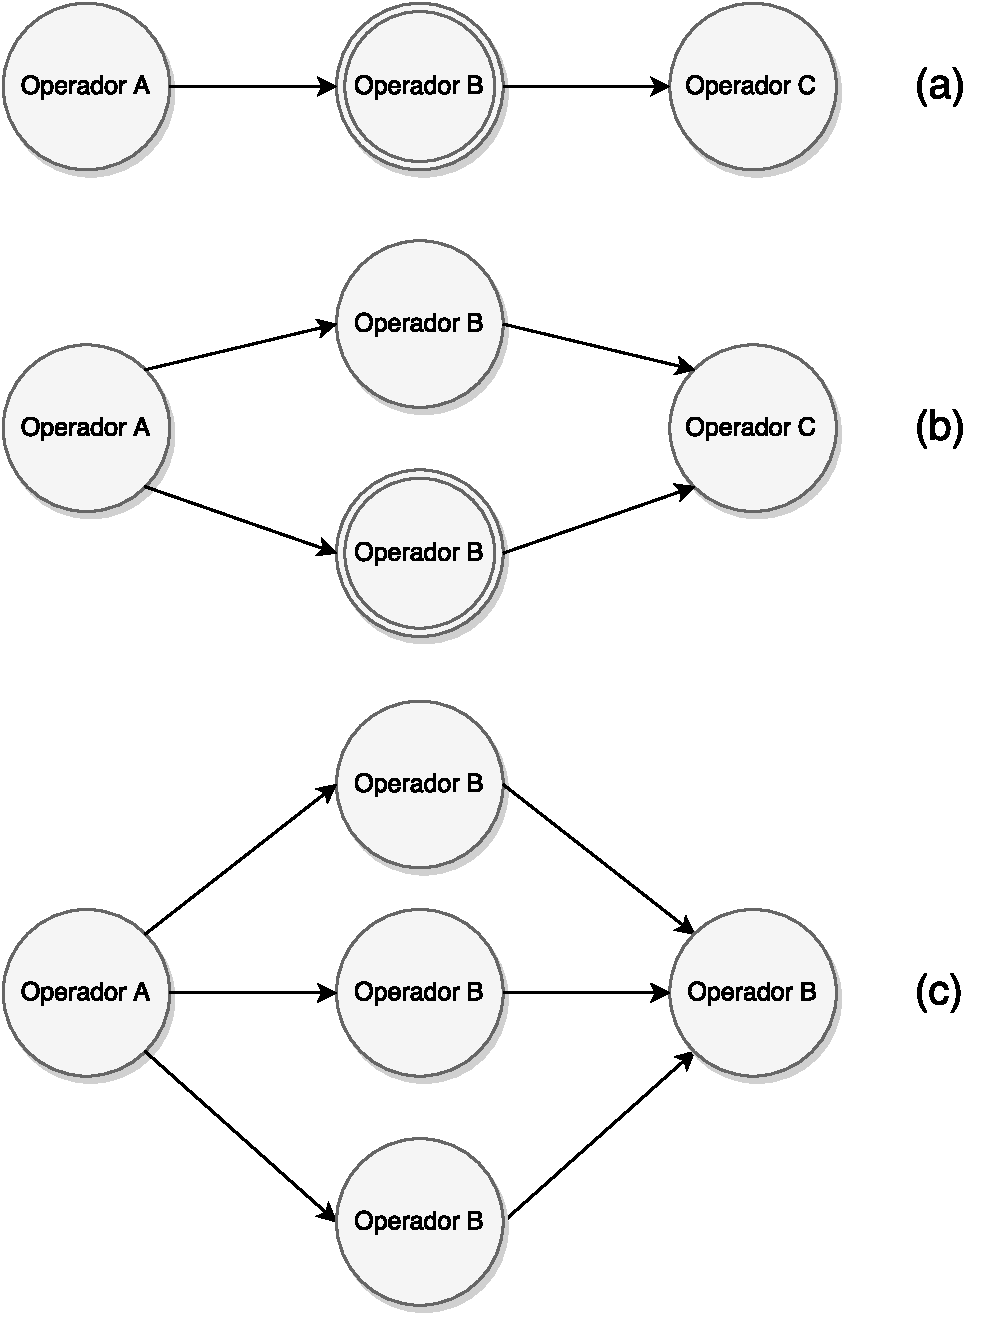
\includegraphics[scale=0.6]{images/EjReplicacion.pdf}
	\caption{Ejemplo de replicación del modelo propuesto.}
	\label{fig:ejReplicacion}
\end{figure}

%Para el diseño del sistema, era necesario contar con un umbral que determinara cuando el operador está o no sobrecargado, por lo que para esto se utilizaron conceptos de teoría de colas \citep{bose2013introduction}. Como los SPS están orientados en grafos, se posee tanto la tasa de llegada ($\lambda$) como la tasa de procesamiento ($\mu$) para cada uno de los operadores, como se ve representando en la Figura \ref{fig:analisisTeoriaColas}, donde la tasa de procesamiento de un operador es la misma tasa de llegada del siguiente operador en el grafo. Utilizando este tipo de conceptos, para cada operador se calculó la tasa de procesamiento ($\rho$), la cual esta definida por la tasa de llegada, la tasa de procesamiento y la cantidad de servicios disponibles en el sistema ($\rho = \frac{\lambda}{\mu \rho}$), cuyo valor nos indica el rendimiento del operador en cierta período de tiempo.

Para la detección del nivel de carga de un operador es necesario contar con un modelo basado en umbrales que permita determinar cuando está o no sobrecargado un operador. Para modelar esta situación se utilizan conceptos de teoría de colas \citep{bose2013introduction}. Dado que los SPS utilizan un paradigma orientado a grafos, se puede obtener tanto la tasa de llegada ($\lambda$) como la tasa de procesamiento ($\mu$) de cada uno de los operadores que lo componen, como se ve representando en la Figura \ref{fig:analisisTeoriaColas}. Aquí la tasa de procesamiento de un operador influye directamente en la tasa de llegada del siguiente operador en el grafo. Al utilizar estos conceptos, se calcula la tasa de rendimiento ($\rho$), la cual está definida por la tasa de llegada, de procesamiento y la cantidad de réplicas del operador ($\rho = \frac{\lambda}{s \mu}$), cuyo valor representa el factor de utilización del sistema, donde se define un sistema estable si y sólo si $\rho < 1$.

\begin{figure}[!hb]
	\centering
		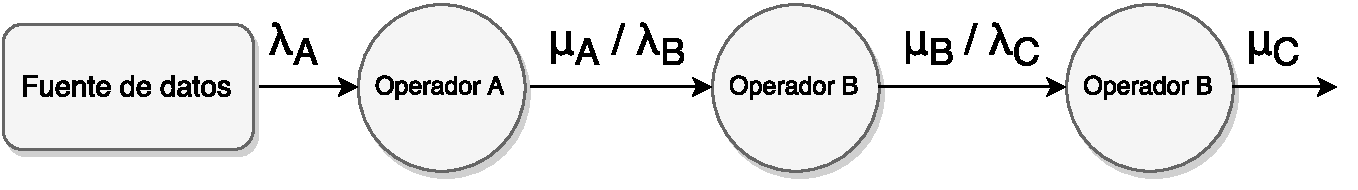
\includegraphics[scale=0.6]{images/AnalisisTeoriaColas.pdf}
	\caption{Enfoque de un SPS con conceptos de teoría de colas.}
	\label{fig:analisisTeoriaColas}
\end{figure}

Tomando en consideración el enfoque dinámico en el algoritmo de balance de carga y la elasticidad que se pretende por parte del modelo, es que se han tratado tres posibles estados en el sistema: ocioso, estable e inestable. El primer estado corresponde a un exceso en la cantidad de recursos asignados. El segundo está definido por el rendimiento óptimo del sistema. Y por último, el tercero hace referencia a un sistema sobrecargado, donde es necesario una mayor cantidad de recursos por parte de éste. Los posibles estados de cada operador son la base para el análisis y predicción de la carga del modelo propuesto.

Para el modelo se consideraron dos tipos de algoritmos: predictivo, enfocado en el futuro basado en la historia del operador, y reactivo, analizando el comportamiento del momento. Este diseño tiene la finalidad de analizar dos factores: los \textit{peaks} existentes en la historia del operador, dado el algoritmo predictivo, y analizar el comportamiento en el momento, haciendo uso del algoritmo reactivo, de tal manera de solucionar los comportamientos que no son detectados con la predicción.

Es importante denotar que dependiendo del tipo de caso es que un algoritmo va a funcionar mejor. Por ejemplo, si existe una variación muy alta en un período de tiempo considerable, el algoritmo predictivo puede detectar este tipo de \textit{peaks}. De esta manera, la predicción es más asertiva que el análisis en el momento. Pero en casos que no suceda lo anterior, y sólo hayan variaciones en ciertos instantes de la ejecución, se encuentra el algoritmo reactivo para analizar el estado del operador.

Además de lo anterior, se considera que es necesario trabajar con los dos algoritmos en temporalidades distintas, es decir, en cierto período de tiempo se utiliza el reactivo y en otro el predictivo. Esto quiere decir que mientras se obtienen las $n$ muestras para realizar el cálculo de predictivo, el algoritmo reactivo está realizando un análisis de los distintos operadores.

%Al diseñar un sistema que pudiera lidiar con dos tipos de algoritmos, era necesario considerar un algoritmo que pudiera administrar la cantidad de cargas, con tal utilizar el algoritmo necesario según el período existente en una ventana de tiempo, como también la cantidad de réplicas que deben aplicarse.

Como se diseñaron dos tipos de algoritmos que se complementan, es necesario considerar un mecanismo que administre cual de los dos algoritmos se va a utilizar según el período analizado, como también la cantidad de réplicas que deben crearse o eliminar según el resultado del algoritmo utilizado.

Dado lo anterior, se ha diseñado un modelo elástico con cuatro componentes: monitor de carga, analizador de carga, predictor de carga y administrador de réplicas, que se presenta en la Figura \ref{fig:componentesSistemas}.

\begin{figure}[ht!]
  \centering
    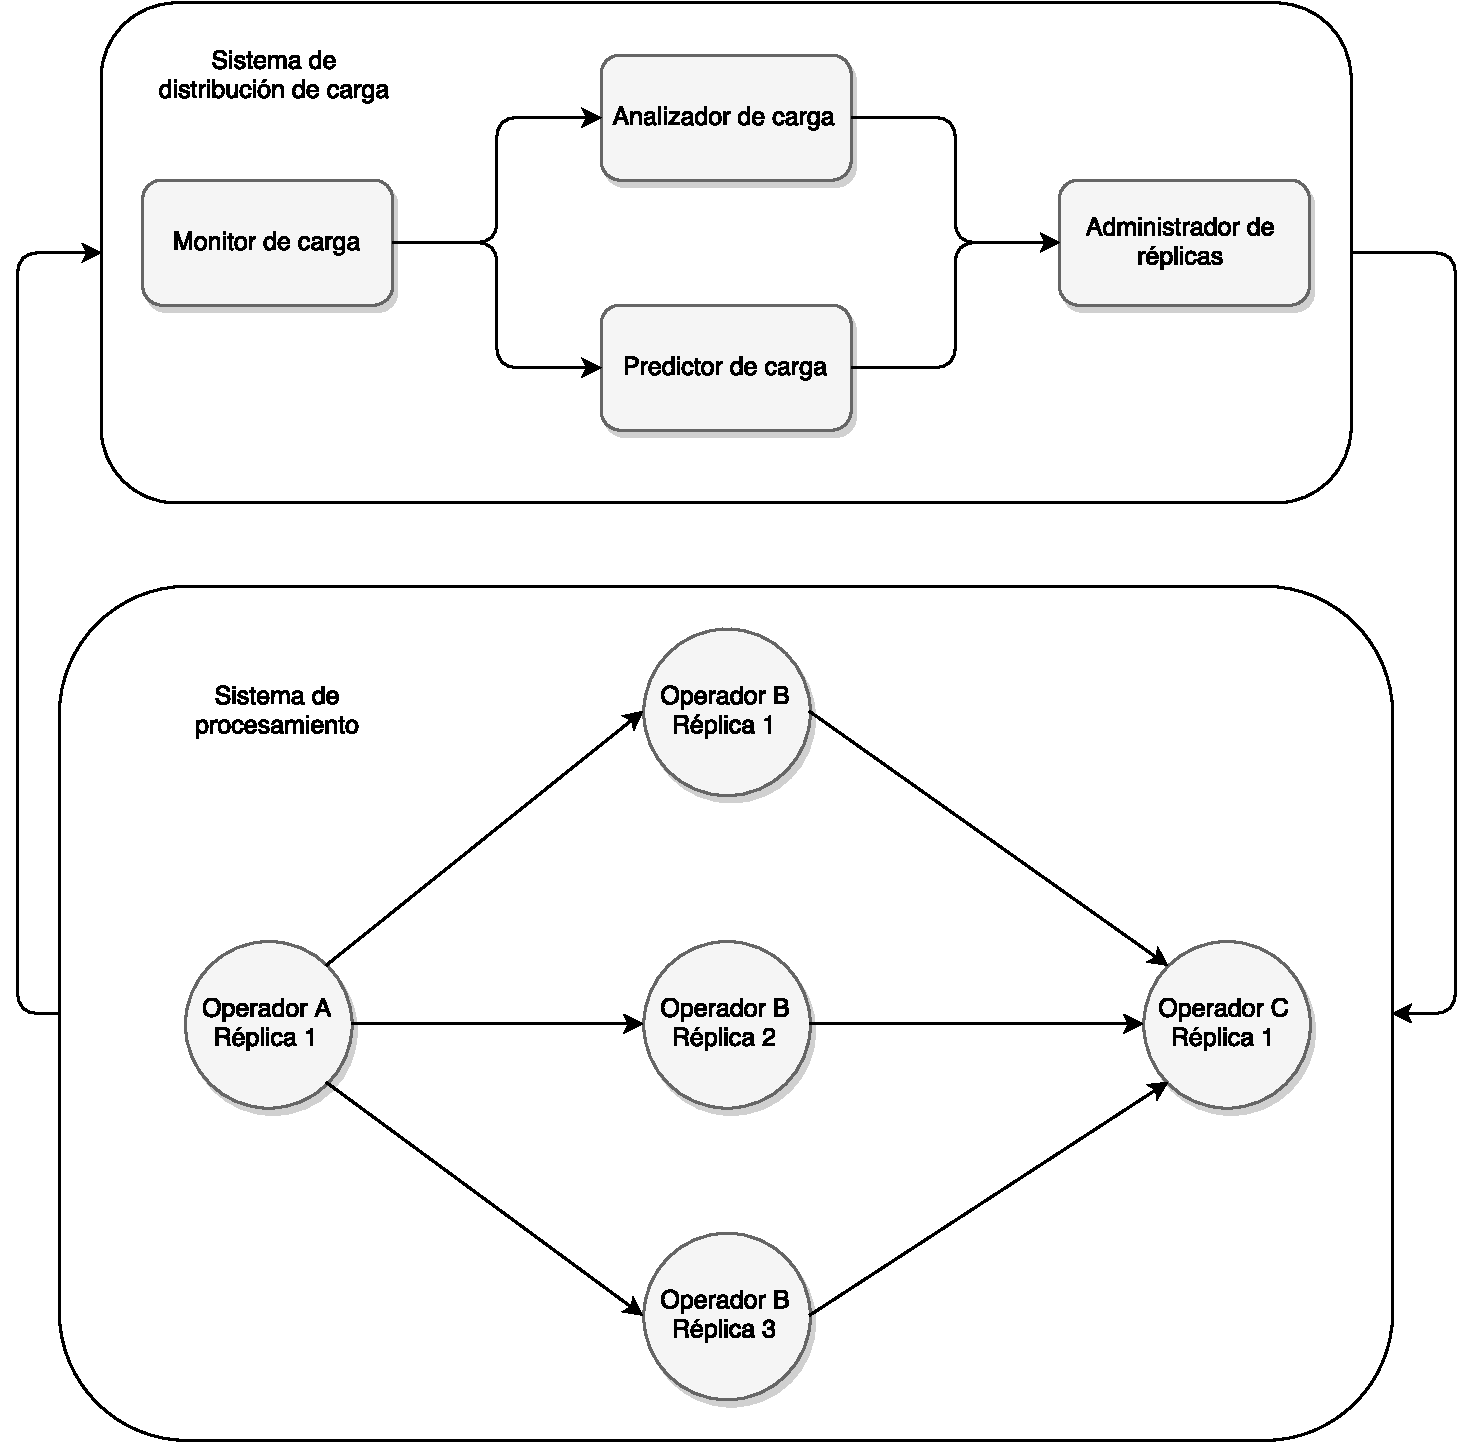
\includegraphics[scale=0.5]{images/Diagrama.pdf}
  \caption{Estructura del modelo elástico.}
  \label{fig:componentesSistemas}
\end{figure}

\paragraph{Monitor de carga:} está encargado de recolectar las estadísticas del sistema, tanto para el algoritmo reactivo, como para el historial del algoritmo predictivo.

\paragraph{Analizador de carga:} analiza la cantidad de carga de un operador en un período de tiempo determinado según el algoritmo reactivo, y respecto a esto se indica el estado del operador. Para esto, se considera la tasa de rendimiento del operador, y según el valor que posea se determina el estado, el cual puede ser ocioso, estable o inestable.

\paragraph{Predictor de carga:} es el módulo del algoritmo predictivo, que analiza la historia de un operador en una ventana de tiempo determinada, utilizando como muestra la tasa de rendimiento del operador, para posteriormente realizar una cadena de Markov según las variaciones del sistema. Posteriormente, para la predicción de la carga del operador, se calcula la distribución estacionaria \citep{Papoulis1984}, el cual entrega la probabilidad que el operador se encuentre en cada uno de los posibles estados.

\paragraph{Administrador de réplicas:} se encarga de determinar cual es el algoritmo a utilizar en cada período de tiempo, ya sea reactivo o predictivo, y la administración de las réplicas utilizando como entrada la información prevista por el analizador y predictor de carga.

\vspace*{0.5cm}

En las siguientes secciones se profundiza en el diseño propuesto para cada uno de estos módulos.

\section{Recolección de los datos}
%Como se había mencionado anteriormente, el monitor de carga está encargado de recolectar la tasa de rendimiento de cada uno de los operadores, tanto del historial como los datos en el momento. Para esto, se consideró una ventana de tiempo de 1 segundo para la recolección del historial, y 5 segundos para el análisis del operador en el momento.

Como se había mencionado anteriormente, el monitor de carga está encargado de recolectar los datos necesarios para el funcionamiento del modelo elástico, tanto el historial para el algoritmo predictivo, como la tasa de rendimiento para el algoritmo reactivo.

La recolección de muestras para el algoritmo predictivo se realiza cada un segundo, debido que se considera tiempo suficiente para obtener una muestra representativa del operador. De esta manera, se espera que existan $n$ muestras para que se ejecute el algoritmo predictivo, por lo que existe una ventana de tiempo $T_p$ entre cada ejecución del algoritmo. La cantidad de muestras fue determinado según la literatura, debido que se considera un número apropiado para realizar una predicción del operador \citep{GongGW10}.

%Analizar con más detalle el tema de mu, porque quizá es erróneo lo descrito aquís
Por otra parte, para la obtención de muestras para el algoritmo reactivo, se consideran muestras obtenidas en períodos de $T_r$. La muestra está compuesta por la tasa de rendimiento del operador en ese período, la cual es utilizada por el algoritmo reactivo para determinar el estado del operador según los umbrales propuestos. Dentro de las consideraciones realizadas para la recolección de datos para el algoritmo reactivo, está el considerar que la tasa de procesamiento ($\mu$) es homogénea con el transcurso del tiempo, considerando que los datos procesados son homogéneos, por lo tanto, se considera un valor promedio de la tasa de procesamiento según los primeros datos procesados. 

Cabe destacar que cuando el algoritmo predictivo se ejecuta, no es necesaria la recolección de los datos del período, debido que el algoritmo reactivo no se ejecuta en el mismo período que el predictivo. Sólo la recolección del historial es realizada en todo momento, dado que estás son guardadas para posteriormente ser analizadas por el algoritmo predictivo. Debido a los algoritmos utilizados, es que se ha considerado ventanas de tiempo de un segundo para la recolección de muestras para el análisis predictivo, y $T_p$ para el análisis reactivo.

\section{Algoritmo reactivo}
El diseño del algoritmo reactivo se basa en el análisis del estado del operador en un período determinado, siendo definido su estado por una variable del operador, el cual depende del rango en que se encuentre dado los umbrales que se establecen. Este diseño analiza según la tasa de rendimiento ($\rho$), donde el estado del operador depende del valor que éste posea según los parámetros del algoritmo.

En el Algoritmo \ref{alg:reactive} se presenta el algoritmo que analiza el estado de un operador según su tasa de rendimiento; en el caso que sea mayor a 1, su estado es inestable, menor a 0.5, significa que está en estado ocioso, y en otro caso, significa que está estable. Estos datos posteriormente son considerados por el administrador de réplicas, el cual analiza el comportamiento que debe tener el sistema según lo indicado por el algoritmo.

\begin{algorithm}[!ht]
	\caption{Algoritmo reactivo del modelo elástico.}
	\label{alg:reactive}
	\begin{algorithmic}[1]
	\REQUIRE Tasa de procesamiento $\rho$ del operador $\phi$.
	\ENSURE Estado del operador, donde -1 significa estado ocioso, 0 estable y 1 inestable.
	\IF {$\rho_\phi > 1$}
		\RETURN{1}
	\ELSIF {$\rho_\phi < 0.5$}
		\RETURN{-1}	
	\ELSE
		\RETURN{0}
	\ENDIF
	\end{algorithmic}
\end{algorithm}

En la Figura \ref{fig:umbrales} se observa el estado de un operador según la tasa de procesamiento. En los primeros 90 segundos la tasa del operador es mayor al límite superior, lo cual indica que el sistema es inestable, es decir, el operador posee sobrecarga. Posteriormente, en el segundo 50, la tasa de rendimiento empieza a disminuir, ya sea por una optimización sobre los recursos lógicos o una disminución de la tasa de llegada, por lo que ahora el operador ya no se encuentra sobrecargado (inestable), sino que se encuentra entre el límite inferior y superior, cuyo rango define al operador como un sistema estable.

\begin{figure}[ht!]
  \centering
    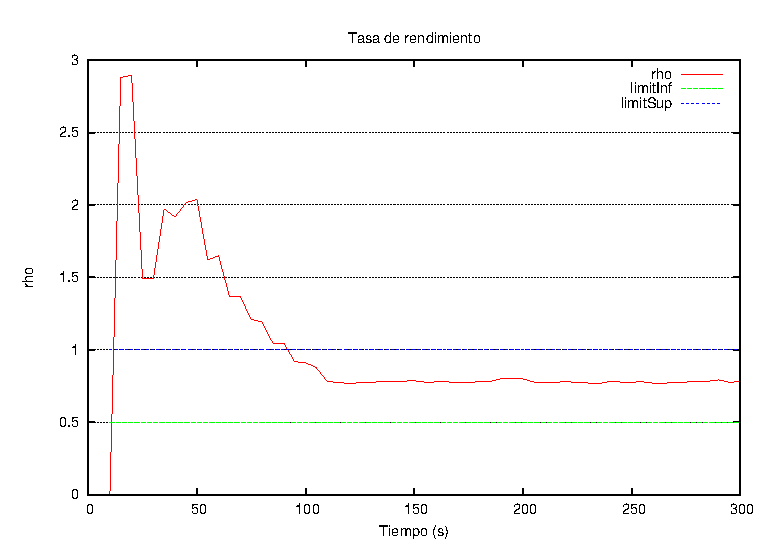
\includegraphics[scale=0.8]{images/Umbrales.eps}
  \caption{Comportamiento de la tasa de procesamiento de un operador.}
  \label{fig:umbrales}
\end{figure}


\section{Algoritmo predictivo}
Para la confección del algoritmo predictivo se ha realizado un análisis según las cadenas de Markov \citep{ching2006markov}, por lo que se tuvieron que seguir las siguientes etapas:

\begin{itemize}
	\item Definir muestras en tiempos discretos, las cuales cambian con el tiempo según un proceso estocástico. Las muestras se definieron como la tasa de procesamiento ($\rho$) del operador, la cual dependiendo de su valor, otorgar un estado al operador.
	\item Determinar los estados finitos que se utilizan para la conformación de la cadena, que son los estados que se puede encontrar el operador: ocioso, estable o inestable.
	\item Obtener una cantidad representativa de muestras para la construcción de la cadena de Markov en el período analizado. Estas muestras son independientes entre un período y otro, por lo que los valores de la cadena de Markov cambian en cada período de tiempo. %Para la implementación del algoritmo, se ha considerado cien muestras por cada período, cuyos intervalos de tiempo son de cien segundos, valor establecido en base al trabajo de \citep{GongGW10}.
\end{itemize}

Tomando las bases anteriores, se ha diseñado una cadena de Markov en base a tres posibles estados: ocioso, estable e inestable, como se muestra en la Figura \ref{fig:cadenaMarkovPredictiva}. Cada uno de los estados posee una probabilidad de transición hacia algún estado, cuyas probabilidades están definidas por las muestras obtenidas en el período de tiempo analizado.

\begin{figure}[ht!]
  \centering
    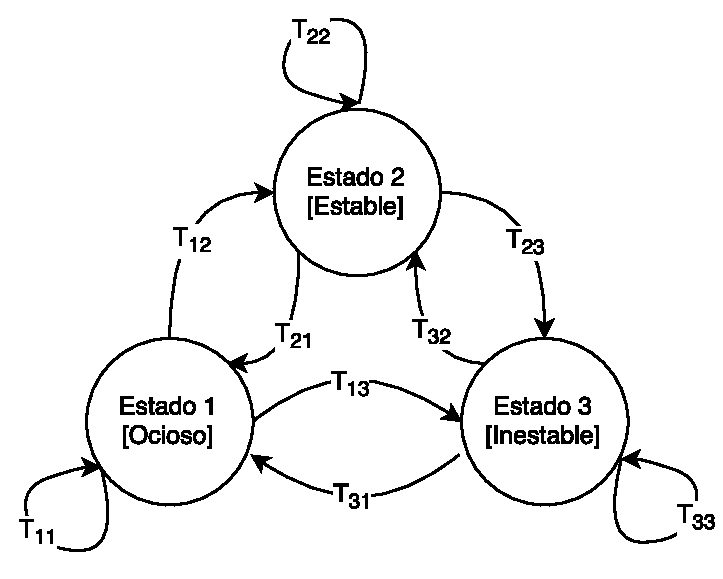
\includegraphics[scale=0.75]{images/CadenaMarkovPredictiva.pdf}
  \caption{Cadena de Markov dado el modelo propuesto del sistema.}
  \label{fig:cadenaMarkovPredictiva}
\end{figure}

%Por lo tanto, para cada operador existe una cadena de Markov según la historia existente en una ventana de tiempo. Para la generación de esta cadena de Markov, se puede ver en el Apéndice \ref{apendice:matrizTransicion} el algoritmo que crea la matriz de transición según el historial del operador, la cual corresponde a la tasa de rendimiento recolectada cada un segundo en la última ventana de tiempo del operador analizado. En la Ecuación \ref{eq:matrizTransicionPredictive} se puede ver la matriz de transición que se obtiene de la cadena de Markov de la Figura \ref{fig:cadenaMarkovPredictiva}, la cual posee una probabilidad de transición desde cada uno de los estado a otro existente.

Por lo tanto, para cada operador se construye una cadena de Markov según el historial obtenido en la ventana de tiempo $T_p$. Para la conformación de la cadena de Markov se ha considerado las muestras de la historia de los operadores, por lo que el comportamiento del estado entre una muestra a otra representa una transición, las cuales dan origen a la matriz de transición. En el Anexo \ref{apendice:matrizTransicion} se presenta el algoritmo que se ha empleado para construir esta matriz. En la ecuación \ref{eq:matrizTransicionPredictive} se muestra la matriz de transición que se obtiene de la cadena de Markov de la Figura \ref{fig:cadenaMarkovPredictiva}.

\begin{equation} \label{eq:matrizTransicionPredictive}
	P =
	\begin{bmatrix}
		T_{1,1} & T_{1,2} & T_{1,3} \\
		T_{2,1} & T_{2,2} & T_{2,3} \\
		T_{3,1} & T_{3,2} & T_{3,3}
	\end{bmatrix}	
\end{equation}

Obtenida la matriz de transición se puede calcular la distribución estacionaria de la cadena de Markov, la cual indica las probabilidades de que en el futuro el operador esté en cada uno de los posibles estados, ya sea ocioso, estable o inestable. Para este cálculo se utiliza la ecuación de Chapman-Kolmogórov \citep{Papoulis1984} descrita en la Sección \ref{subsec:cadenaMarkov}.

El Algoritmo \ref{alg:distEstacionaria} describe el cálculo de la distribución estacionaria, cuya entrada es la matriz de transición de un operador del SPS. 

\begin{algorithm}[!t]
	\caption{Cálculo de la distribución estacionaria de la cadena de Markov de un operador $\phi$.}
	\label{alg:distEstacionaria}
	\begin{algorithmic}[1]
	\REQUIRE $\Gamma$ Matriz de transición del operador $\phi$, $\upsilon$ cantidad de iteraciones deseadas y última muestra $m$ de las muestras de $\rho$
	\ENSURE $\Delta$ Distribución estacionaria de la cadena de Markov del operador $\phi$.
	\STATE $i \leftarrow 0$ \COMMENT {Estado inicial de iteración}
	\IF {$\rho_m < 0.5$}
		\STATE {$i \leftarrow 0$}
	\ELSIF {$0.5 \leqslant \rho_m \leqslant 0.5$}
		\STATE {$i \leftarrow 1$}
	\ELSE
		\STATE {$i \leftarrow 2$}
	\ENDIF
	
	\STATE $\tau \leftarrow Arreglo[3]$ \COMMENT {Contador para la normalizaci\'on de los datos}
	\FOR {$k=0$ a $\upsilon$}
		\STATE $u = randomUniform(0,1)$
		\STATE $\sigma = 0$
		\FOR {$j=0$ a $3$}
			\STATE $\sigma = \sigma + \Gamma_{i,j}$
			\IF {$u \leqslant  \sigma$}
				\STATE $\tau_{j}++$
				\STATE $i \leftarrow j$
				\STATE \textbf{break}
			\ENDIF
		\ENDFOR
	\ENDFOR

	\STATE $\Delta \leftarrow Arreglo[3]$ \COMMENT {Distribución estacionaria de la cadena de Markov del operador $\phi$}
	\FOR{$k=0$ a $3$}
		\STATE $\Delta_{k} \leftarrow \nicefrac{\tau_{k}}{\upsilon}$
	\ENDFOR	
	
	\RETURN $\Delta$
	
	\end{algorithmic}
\end{algorithm}

%Antes de realizar el cálculo, es importante analizar si efectivamente existen transiciones en todos los estados, debido a que existe la posibilidad que no haya una transición a un estado en particular en un período de tiempo. Por ejemplo, puede ocurrir que en una ventana de tiempo nunca se ha alcanzado el estado ocioso en el sistema, pero si el estable o inestable. Como el cálculo de la distribución estacionaria requiere un estado de inicio, se ha verificado si efectivamente existe o no el estado, y en caso no existir, el estado de inicio es alguno existente.

Antes de realizar el cálculo, es importante definir el estado inicial para el proceso de iteración. Es por esto que se escoge la última muestra obtenida, y según el estado que ésta se encuentre es el estado inicial que se utiliza para el cálculo de la distribución estacionaria.

La cantidad de iteraciones $\upsilon$ que debe realizarse para el cálculo correspondiente, es un parámetro entrada del algoritmo. Es importante destacar que entre mayor es la cantidad de iteraciones, mayor es la precisión del valor predicho. Esto implica a su vez un mayor tiempo de cómputo, por lo que se ha considerado un punto medio, de tal manera de lograr un bajo margen de error, pero con bajo costo en el tiempo de ejecución. %La cantidad de iteraciones escogida para la implementación fue de 100.000.

%\vspace{-2cm}

Obtenida la distribución estacionaria, se procede a analizar las probabilidades obtenidas y como es el comportamiento del operador. Para esto, se ha considerado que las probabilidades tengan una desviación estándar superior a 0.25, lo que indica que la probabilidad mayor de la distribución estacionaria no posea incertidumbre. En el caso que no supere la desviación estándar, puede ser que dos probabilidades sean muy parecidas y la probabilidad no sea un comportamiento determinante \citep{soong2004fundamentals}. El Algoritmo \ref{alg:predictive} detalla el análisis que se realiza a la distribución estacionaria, siendo en primer lugar el análisis estadístico de las probabilidades, y en segundo lugar la obtención del estado con mayor valor de las probabilidades, retornando finalmente el estado del operador. Cabe destacar que el primer estado se ha considerado ocioso, el segundo estable, y el tercero inestable.

\begin{algorithm}[t]
	\caption{Algoritmo predictivo del modelo elástico.}
	\label{alg:predictive}
	\begin{algorithmic}[1]
	\REQUIRE$\Delta$ Distribución estacionaria de la cadena de Markov del operador $\phi$.
	\ENSURE Estado a futuro del operador, donde -1 significa estado ocioso, 0 estable y 1 inestable.
	\IF {$\sigma(\Delta_1,\Delta_2,\Delta_3) > 0.25$ \COMMENT {Desviaci\'on est\'andar de las probabilidades de la distribuci\'on estacionaria}} 
		\STATE $i \leftarrow getStateMax(\Delta)$ \COMMENT {Obtención del estado con mayor probabilidad}
		\IF {$i=1$}
			\RETURN -1
		\ELSIF {$i=2$}
			\RETURN 0			
		\ELSE
			\RETURN 1
		\ENDIF
	\ENDIF
	
	\RETURN 0
	
	\end{algorithmic}
\end{algorithm}

\section{Administración del sistema}

El último componente del modelo es el administrador de réplicas, cuya función es administrar la cantidad de réplicas en cada uno de los operadores según los recursos disponibles en el sistema y según el estado que adopte un operador, ya sea a futuro o en el momento.

%Para esto, se ha diseñado un administrador que ejecuta uno de los algoritmos (reactivo o predictivo) según el período del ciclo que se encuentre el sistema. Cada ciclo posee 20 períodos, donde los primeros 19 corresponden al algoritmo reactivo y el último corresponde al algoritmo predictivo. Cada período posee un intervalo de 5 segundos, de esta manera, cada ciclo tiene un intervalo de 100 segundos, la cantidad necesaria para obtener las muestras para el algoritmo predictivo, suponiendo que cada muestra es obtenida cada 1 segundo.

Para esto, se ha diseñado un administrador que ejecuta el algoritmo reactivo en un período de $T_r$ y el algoritmo predictivo en un período de $T_p$. Cabe destacar, que la ventana de tiempo utilizada para el algoritmo reactivo es mayor que la del predictivo, esto debido que uno analiza el comportamiento en el momento y otro a futuro según la historia.


\begin{algorithm}[!ht]
	\caption{Administración de réplicas de un operador $\phi$ dado su comportamiento en el modelo elástico.}
	\label{alg:administracion}
	\begin{algorithmic}[1]
	\REQUIRE Operador $\phi$ a analizar y $\iota$ período en que se encuentra el modelo elástico.
	\ENSURE Cantidad de réplicas a modificar del operador.	
	
	\IF {$\iota$ es $T_p$}
		\STATE $\delta_{\iota} \leftarrow AlgoritmoPredictivo(\phi)$
		\IF {$\delta_{\iota}$ es estado inestable}
			\IF {No excede la cantidad máxima de réplicas en el sistema}
				\RETURN Crear $\theta$ réplicas del operador $\phi$
			\ENDIF
		\ELSIF {$\delta_{\iota}$ es estado ocioso}
			\RETURN Remover $\theta$ réplicas del operador $\phi$
		\ENDIF
	\ELSE[$\iota$ es $T_r$]
		\STATE $\delta_{\iota} \leftarrow AlgoritmoReactivo(\phi)$
		\IF {$\delta_{\iota}$ \AND $\delta_{\iota-1}$ son estado inestable}
			\IF {No excede la cantidad máxima de réplicas en el sistema}
				\STATE $\delta_{\iota} \leftarrow \text{estado estable}$ 
				\RETURN Crear $\omega$ réplica del operador $\phi$
			\ENDIF
		\ELSIF {$\delta_{\iota}$ \AND $\delta_{\iota-1}$ son estado ocioso}
			\STATE $\delta_{\iota} \leftarrow \text{estado estable}$ 
			\RETURN Remover $\omega$ réplica del operador $\phi$
		\ENDIF 
	\ENDIF
	
	\RETURN No hacer nada al operador $\phi$
	
	\end{algorithmic}
\end{algorithm}

En el Algoritmo \ref{alg:administracion} está el procedimiento de administración, donde primero se analiza que tipo de algoritmo se debe ejecutar según el período del ciclo. En caso de ejecutarse el módulo predictivo, se analiza cual es la predicción, por lo que si el estado es ocioso el sistema disminuye la cantidad de réplicas y si es inestable las aumenta. Como el proceso de predicción se realiza con menor frecuencia y posee mayor cantidad de cómputo, se ha considerado que se debe crear o remover una mayor cantidad de réplicas que en el módulo reactivo, aprovechando así el análisis de la historia del operador. Por otra parte, de realizarse el algoritmo reactivo se analiza si existen dos alertas consecutivas del mismo estado del operador, ya sea ocioso o inestable, y de ser así, realizar una modificación a la cantidad de réplicas del operador. Además, se cambia el estado actual del operador a estable, de tal manera de no considerar ese período para el próximo análisis reactivo. Esto se realiza para dejar un margen de descanso al algoritmo reactivo

Dentro de las consideraciones que se han tenido para el diseño del administrador, es limitar la cantidad máxima de réplicas que pueden realizarse. Esto se debe a que una de las limitantes de este trabajo es que se ha  utilizado solo una máquina, y por ende la cantidad de recursos son limitados, por lo que al aumentar la cantidad de réplicas indefinidamente genera una sobrecarga en los recursos disponibles por parte de la máquina.